\setcounter{chapter}{6}

\chapter{Advanced Group Theory}

\section*{April 26th, 2023}

\setcounter{topic}{33}
\topic{Isomorphism Theorems}

% We have two topics in advanced group theory. Jordan-Hölder theorem, and the Sylow theorems. They are related to classification theory. Jordan-Hölder theorem relates to normal subgroups and quotient groups. Sylow theorems relate to group actions.

\thm. \note{First Isomorphism Theorem} Let \(\varphi : G \ra G'\) be a group homomorphism. Then \(\mu : G/ \ker \varphi \ra \im \varphi\) defined as
\[
    \mu(x \ker\varphi) = \varphi(x), \quad (x \in G)
\]
is an isomorphism, and \(G / \ker \varphi \simeq \im \varphi\).
\[
    \begin{tikzcd}
        G \arrow{rr}{\varphi} \arrow[swap]{dr}{\pi} & \arrow[d, phantom, "\circlearrowright"]& \im \varphi \\
        & G/\ker\varphi \arrow[dashed,swap]{ur}{\mu} &
    \end{tikzcd}
\]

\lemma. Let \(N \nsub G\) and \(\gamma : G \ra G / N\) be a canonical homomorphism. Then
\[
    \varphi: \{M \nsub G : N \leq M\} \ra \{K \nsub G/N\}
\]
defined as \(\varphi(M) = \gamma(M)\) is a bijection.

\pf Since \(\gamma\) is a epimorphism, if \(M \nsub G\), then \(\varphi(M) = \gamma(M) \nsub \gamma(G) = G/N\). We next show that \(\varphi\) is a bijection. \(\varphi(L) = \varphi(M)\), then \(\gamma(L) = \gamma(M)\) so \(L = M\). This works because \(N \leq M\) and \(\gamma\inv(\gamma(M)) = M\). Also, for \(K \nsub G/N\), \(\varphi(\gamma\inv(K)) = K\). \qed

\recall We proved a part of this when we proved that if \(M\) is a maximal normal subgroup, then \(G/M\) is simple.

\notation For \(H, N \leq G\), define \(H \vee N = \span{H, N}\).

\lemma.
\begin{enumerate}
    \item If \(N \nsub G\) and \(H \leq G\), \(HN = NH \leq G\). i.e. \(H \vee N = HN = NH\).
    \item If \(N \nsub G\) and \(H \nsub G\), then \(H \vee N = HN \nsub G\).
\end{enumerate}

\pf \\
\note{1} Let \(h_1n_1, h_2n_2 \in HN\) for \(h_i \in H, n_i \in N\). Since \(N \nsub G\), \(\exists n_3 \in N\) such that \(h_1 n_1 h_2 n_2 = h_1 h_2 n_3 n_2\), which is an element of \(HN\). Check that \(e \in HN\), \((hn)\inv \in HN\).

\note{2} For \(g \in G\), we show that \(ghng\inv \in HN\) for \(h \in H\), \(n \in N\). Since both subgroups are normal, there exists \(h' \in H\), \(n' \in N\) such that \(hng\inv = g\inv h' n'\). Then \(ghng\inv = (gg\inv)h'n' \in HN\). \qed

\medskip

\thm. \note{Second Isomorphism Theorem} If \(H \leq G\) and \(N \nsub G\),
\[
    \frac{HN}{N} \simeq \frac{H}{H\cap N}.
\]
\begin{center}
    \begin{tikzpicture}
        \node (H) at (0, 0) {\(H\)};
        \node (HN) at (3, 0) {\(HN\)};
        \node (HoverHcapN) at (0, -2.5) {\(\dfrac{H}{H \cap N}\)};
        \node (HNoverN) at (3, -2.5) {\(\dfrac{HN}{N}\)};

        \draw[->] (H) -- (HN) node[midway,above,scale=0.7] {\(\imath\)};
        \draw[->] (HN) -- (HNoverN) node[midway,right,scale=0.7] {\(\pi'\)};
        \draw[->] (H) -- (HoverHcapN) node[midway,left,scale=0.7] {\(\pi\)};
        \draw[->] (HoverHcapN) -- (HNoverN) node[midway,below,scale=0.7] {\(\bar{\jmath}\)} node[midway,above,scale=0.7] {\(\simeq\)};
        \draw[->] (H) -- (HNoverN) node[midway,above right,scale=0.7] {\(\jmath\)};

        \node[scale=0.6] at (0.7, -1.6) {\(\circlearrowright\)};
        \node[scale=0.6] at (2.3, -0.6) {\(\circlearrowright\)};
    \end{tikzpicture}
\end{center}

\pf We first have to check that \(N \nsub HN\) and \(H\cap N \nsub H\). (Check!)

Consider \(\gamma : G \ra G/N\). It is clear that \(\gamma\) is surjective.
\begin{itemize}
    \item \(\gamma \mid_H: H \ra \gamma(H)\)
    \item \(\gamma \mid_{HN}: HN \ra \gamma(HN)\). Actually, \(\gamma(HN) = \gamma(H)\).
\end{itemize}
By the first isomorphism theorem,
\[
    \frac{H}{\ker \gamma\mid_H} \simeq \gamma(H) \simeq \frac{HN}{\ker \gamma \mid_{HN}}.
\]
Now we check that \(\ker \gamma\mid_H = H \cap N\) and \(\ker \gamma\mid_{HN} = N\). This is trivial. \qed

\ex. Let \(G = \Z_{24}\), \(H = \span{4}\), \(N = \span{6}\). Then
\[
    HN = \{n4 + m6 : n, m \in \Z\} = \span{2}, \quad H\cap N = \span{4}\cap \span{6} = \span{12}.
\]
We see that \(HN / N \simeq H / H\cap N \simeq \Z_3\).

\medskip

\thm. \note{Third Isomorphism Theorem} If \(H, K \nsub G\) and \(K \leq H\),\footnote{This implies that \(K \nsub H\).} then
\[
    G / H \simeq \frac{G/K}{H/K}.
\]

\pf We first have to check that \(K \nsub H\) and \(H/K \nsub G/K\). (Check the first)

Let \(\bar{g} \in G/K\), \(\bar{h} \in H/K\). We show that \(\bar{g} \cdot \bar{h} \cdot \bar{g\inv} \in H/K\), this is trivial. Define
\[
    \varphi : G \overset{\psi_1}{\longrightarrow} G/K \overset{\psi_2}{\longrightarrow} \frac{G/K}{H/K}.
\]
We check that \(\varphi\) is a well-defined group homomorphism, and that \(\varphi\) is surjective, and \(\ker \varphi = H\). Then the result directly follows from the first isomorphism theorem. \qed

\ex. Let \(G = \Z\), \(H = 2\Z\), \(K = 6\Z\). \(G/K \simeq \Z_2\), \(G/K \simeq \Z_6\), \(H/K \simeq \Z_3\). Then \(\Z_2 \simeq \Z_6 / \Z_3\) (abuse of notation) by the third isomorphism theorem.

\topic{Series of Groups}

Given a group \(G\), we want to decompose \(G\) with simpler groups, \(G \leadsto G_1 * G_2 * \cdots * G_k\). We consider a series of normal subgroups,
\[
    \cdots \nsub N_3 \nsub N_2 \nsub N_1 \nsub G.
\]
Then we can consider a sort of a situation like
\[
    G = G/N_1 * N_1 / N_2 * N_2 / N_3 * \cdots
\]
and if each normal subgroup is maximal, then each term is simple! This leads us to the Jordan-Hölder theorem. We will use the second/third isomorphism theorems.


\pagebreak
